% This must be in the first 5 lines to tell arXiv to use pdfLaTeX, which is strongly recommended.
\pdfoutput=1
% In particular, the hyperref package requires pdfLaTeX in order to break URLs across lines.

\documentclass[11pt]{article}

% Remove the "review" option to generate the final version.
% \usepackage[review]{ACL2023}
\usepackage{ACL2023}

% Standard package includes
\usepackage{times}
\usepackage{latexsym}
\usepackage{graphicx}
\usepackage{booktabs}

% For proper rendering and hyphenation of words containing Latin characters (including in bib files)
\usepackage[T1]{fontenc}
% For Vietnamese characters
% \usepackage[T5]{fontenc}
% See https://www.latex-project.org/help/documentation/encguide.pdf for other character sets

% This assumes your files are encoded as UTF8
\usepackage[utf8]{inputenc}

% This is not strictly necessary, and may be commented out.
% However, it will improve the layout of the manuscript,
% and will typically save some space.
\usepackage{microtype}

% This is also not strictly necessary, and may be commented out.
% However, it will improve the aesthetics of text in
% the typewriter font.
\usepackage{inconsolata}

\usepackage{url}


% If the title and author information does not fit in the area allocated, uncomment the following
%
% \setlength\titlebox{<dim>}
%
% and set <dim> to something 5cm or larger.

\title{Investigating Indirect Communication Abilities of Transformer-based LMs}

% Author information can be set in various styles:
% For several authors from the same institution:
\author{Geetansh Saxena \and Maksim Shmalts \\
        University of Tübingen \\
        \texttt{\{geetansh.saxena, maksim.shmalts\}@student.uni-tuebingen.de}}
% if the names do not fit well on one line use
%         Author 1 \\ {\bf Author 2} \\ ... \\ {\bf Author n} \\
% For authors from different institutions:
% \author{Author 1 \\ Address line \\  ... \\ Address line
%         \And  ... \And
%         Author n \\ Address line \\ ... \\ Address line}
% To start a seperate ``row'' of authors use \AND, as in
% \author{Author 1 \\ Address line \\  ... \\ Address line
%         \AND
%         Author 2 \\ Address line \\ ... \\ Address line \And
%         Author 3 \\ Address line \\ ... \\ Address line}

% \author{Geetansh Saxena \\
%   University of Tübingen \\
%   International Studies Computational Linguistics \\
%   \texttt{geetansh.saxena@student.uni-tuebingen.de} \\\And
%   Maksim Shmalts \\
%   University of Tübingen \\
%   Seminar für Sprachwissenschaft \\
%   \texttt{maksim.shmalts@uni-tuebingen.de} \\}
\newcommand{\promptblock}[1]{%
    \parbox{\linewidth}{\raggedright\ttfamily\small #1}
    \vspace{0.5\baselineskip}
}
\begin{document}
\maketitle


\begin{abstract}
Human language understanding relies heavily not only on the linguistic meaning of the perceived language signs, but also on a large set of extra-linguistic notions, beliefs, immediate contextual cues, and much more. Many attempts have been made to build a model of human communication that would include these pragmatic factors. In particular, \citet{achimova-2025} suggest that the choice of the utterance is actively affected by the speaker’s belief about the listener’s opinion on the conversation topic and confirms this hypothesis with experiments with human participants. We aim at investigating to what extent this behavior is transmitted to language models (LMs). We report a noticeable correlation between the size of the model and the extent to which it acquires the investigated behavioral pattern. We find that smaller LMs are incapable of replicating the discussed indirect speech tendency, while larger models show some initial yet promising results in that direction.
\end{abstract}


\section{Introduction}
\label{sec:intro}

Human language understanding relies heavily not only on the linguistic meaning of the perceived language signs, but also on a large set of extra-linguistic notions, beliefs, immediate contextual cues, and much more (\citealt{schubert-1986}, \citealt{wittgenstein-1953}). Correspondingly, the speaker should take these background entities into account in order to produce a text that is intelligible for the listener. Furthermore, an extensive body of literature argues that these factors actively affect the utterance choice of the speaker (see, for example, \citealt{van-dijk-1990}). In particular, a line of works focuses on the social perspective of human communication and argue that social factors can explain different strategies employed by the speakers in different situations. \citet{wittgenstein-1953} introduces the concept of \textit{language game}. He suggests that the speaker produces an utterance that would be most relevant for the listener to build their next utterance on; by exchanging the utterances, the dialogue participants thus approximate the common goal (e.g. exchanging the news or opinions). Developing this concept, \citet{austin-1962} proposes the influential \textit{Speech Act Theory}. This framework assumes that the speaker uses communication to achieve goals in the real world, and so the speaker incorporates their underlying intentions into the utterance by choosing a particular language form. In particular, when direct declaration of the goal might damage the relationship between the dialogue participants, the speaker might prefer an expression that would be socially plausible while keeping the actual intention discoverable by the listener. In Speech Act Theory, such utterances are called indirect. The standard example for an indirect utterance is the question "can you please pass me the salt?". While formally inquiring of the ability of the listener to pass them the salt, the speaker actually asks them to perform the action 'pass the salt'; the indirect utterance is much more polite in this case than the direct "pass the salt". Finally, \citet{grice-1975} concludes that the language game-like goal-centered interchange of utterances constitutes the \textit{cooperative principle} that guides the choice of the utterance in human communication. Following the principle both ensures mutual intelligibility and serve the social purpose.


Many attempts have been made to build a model of human communication that would include (part of) pragmatic factors outlined above (e.g. \citealt{achimova-2022}, \citealt{goodman-2013}). One of the prominent approaches is the \textit{Rational Speech Act framework} \citep{goodman-2012}. The model assigns probabilities to the possible utterances from a fixed set based on their expected informational utility. While accounting for a number of extra-linguistic factors, the original frameworks oversees the social utility, that, as argued by the foundational works outlined above, is a crucial driver of human communication. The extensions of this framework addresses this shortcoming and incorporate the social utility expectancy as one of the variables predicting the utterance choice \citep{carcassi-2023}. While providing a valuable basis for further modeling, the previous of the Rational Speech Act framework fell short to also take into account the listener's opinion, and focused only on the speaker, which again does not fully conform to the language game and cooperative principles.

Conversely, \citet{achimova-2025} suggest that the choice of the utterance is actively affected by the speaker’s belief about the listener’s opinion on the conversation topic. They hypothesize that when the opinions of the participants of the dialogue do not match, the speaker tends to choose utterances that would prioritize not contradicting the listener's opinion rather than expressing own speaker's opinion. They develop a novel model called \textit{AMIC} (Alignment Model of Indirect Communication) that accounts for the match/mismatch of the opinions of the dialogue participants. \citet{achimova-2025} conduct a set of empirical experiments with human participants that support the hypothesis. The key finding of the paper is that \textit{the speakers produce more indirect speech when there is a conflict of opinions}.

Given this promising finding, we aimed at investigating to what extent this behavior is transmitted to language models (LMs)\footnote{In this study, we focused on the latest generative transformer-based language models since they have shown unprecedented advances in language modeling technology.} that have been argued to acquire some patterns of human behavior from the training data \citep{hashemi-2025}. More specifically, we investigated whether LMs acquire the same tendency to incline towards indirect speech when a conflict of opinions is possible. For that purpose, we replicated the original experiments 2 (\textit{Speaker Experiment}) and 3 (\textit{Pragmatic Listener Experiment}) from \citet{achimova-2025}. We utilized LMs of size 360M to 4B parameters to simulate the human participants from the original experiments, and ran a set of statistical test over the experimental outcomes to interpret the results. We found a noticeable correlation between the size of the model and the extent to which it acquires the investigated behavioral pattern. The main finding of our study is that smaller LMs are incapable of replicating the discussed indirect speech tendency, while larger models show some initial yet promising results in that direction.


\section{Methods}
\label{sec:methods}

We structure this section the following way: 1) first, the original experiments are introduced; 2) then, we report the procedure of data collection for reproduction of the experiments; 3) afterwards, we introduce the technical setup for the experimental runs; 4) finally, the experimental workflows are described.

\subsection{Original Experiments}
\label{sec:orig}

The original experiments from \citet{achimova-2025} were designed to evaluate the main hypothesis that humans tend to choose indirect utterances in the situation of possible opinion conflict, as well as compare the empirical data from human participants with the predictions from the AMIC model. The experiments investigated the phenomenon from two perspectives.

In the \textit{Speaker Experiment}, 98 participants were given trials where a topic, the opinions of the speaker and the listener on this topic, and the communicative goal of the speaker were given. Three communicative goals were presented: informational --- directly share the opinion, social --- avoid possible conflict, and mixed --- share the opinion while trying to avoid possible conflict. The goal of the participant was to choose the most appropriate utterance for the speaker from a predefined set, corresponding to possible evaluations of the suggested topic from strongly negative to strongly positive. Thus, the effect of the opinions match/mismatch and the communicative goal on the choice of the utterance was investigated.

The outcome of this experiment demonstrated that the participants indeed conformed to the expected tendency. Even though no significant difference were found between the answers with the mixed and social goals, both these goals gave rise to statistically more indirect speech than the informational goal.

The \textit{Pragmatic Listener} reversed the previous experiment and presented 274 participants with two-turn dialogues where the first and the second speaker shared utterances evaluating a given topic. The goal of the participants was to infer the second speaker's latent opinion based on their response to the first speaker's utterance. The core goal was to verify whether conversational context and perceived communicative goals dynamically influence the interpretation of an utterance. The experiment confirmed that human interpretation dynamically adjusts to the social context of conflict avoidance. 

The AMIC model’s predictions were also collected over the same trials. The study arrived at the conclusion that the AMIC's prediction trend positively correlates to the expirical human data.

% Human participants ($n=274$) were presented with a two-turn dialogue between two individuals whose explicit goal was to exchange opinions but avoid conflict (activating the model's social utility). An example of that two turn dialogue presented to the human participants is presented in image xx. The design manipulated the positivity of the First Speaker's Utterance ($u_{1}$) across the scale, and the Second Speaker's Response ($u_{2}$) used neutral to slightly positive/negative indirect terms. The experiment checked a key monotonicity prediction: that the inferred opinion of $S_{2}$ for a fixed response ($u_{2}$) would be \textbf{negatively correlated} with the positivity of the preceding statement ($u_{1}$). This confirmed that human interpretation dynamically adjusts to the social context of conflict avoidance.


\subsection{Data Collection}
\label{sec:data}

As mentioned in section 1 \nameref{sec:intro}, we replicated (with suitable adjustments wherever necessary) the original experiments with a set of LMs. In doing so, we simulated human participants with LMs by instructing the models to play the role of the experiment participant and presenting them with the same (or highly similar) experimental vignettes.

The original experiments featured 10 distinct topics ranging from politically charged (e.g., \textit{immigration laws}) to social issues (e.g., \textit{animal rights}). These topics provided the conversational context for the dialogues. The speakers latent opinions were formulated on a scale 1 to 5 and were visually represented as a number of hearts corresponding to the opinion from 1 being strongly negative to 5 being strongly positive. For a more pronounced contrast, only 1 or 5 were used as the possible opinions. The resulting utterances featured valuation adjectives. There were 10 possible valuation adjectives, two for each point of the 5-point scale.

For the Speaker Experiment, the combinations of opinion match/mismatch, negative (1) / positive (5) speaker's opinion, and one of the three commutative goals formed a space of 12 possible design cells. For each of the participants, 10 combinations were sampled and were coupled with 10 possible topics randomly. Since answers from 7 participants were discarded, 91 $\times$ 10 = 910 vignettes were generated for the experiments in total.

For the Pragmatic Listener experiment, 32 unique adjective combinations corresponding to combinations of the utterances of the first and the second speaker were collected. For each participants, 6 trials with randomly sampled combinations were run. Data from 12 participants were excluded from the analysis, and so 274 $\times$ 6 = 1644 vignettes were generated.

The experimental vignettes for the two experiments are accessible under \url{https://osf.io/nvrh9?view_only=86a0546483354ef49ad37c58e2cb4f0f} and \url{https://osf.io/mbsk9?view_only=86a0546483354ef49ad37c58e2cb4f0f}, respectively.

% The core ambiguity originated from the 32 unique adjective combinations designed to test the limits of polite interpretation. These 32 combinations were created by crossing two distinct sets of adjectives ($6\times 6$), and then systematically excluding the 4 pairs where the First Speaker's adjective ($u_{A}$) perfectly matched the Second Speaker's reply ($u_{B}$), such as "poor" vs. "poor."

For our experimentations with LMs, we reproduced the vignettes for the two experiments as input prompts for LMs. For the Speaker Experiment, the original vignettes were reproduced, resulting in 910 vignettes. Each vignette featured the participant profile for the LM to model. Our approach to collection of the data for the Pragmatic Listener Experiment was slightly different: we crossed the 32 possible adjectives combinations with the 10 topics, thus producing 320 vignettes, to cover the entire possible combination space. These vignettes were de-personified. With that, we wanted to investigate the effect of space exploration as well as profile assignment on the LMs' judgements.

Additionally, we duplicated the obtained vignette prompts with a small difference: instead of the hearts as used in the original experiments, we inserted plain text there (e.g. "strongly positive"). That served the purpose to test the robustness of LMs' interpretation against abstractness of the opinion formulation.

% We designed two sets of 320 prompts for each of the 10 topics:

% \begin{itemize}
%     \item \textbf{Plain Mode (320 Prompts):} The system prompt used plain text to describe the opinion scale ("Strongly Negative to Strongly Positive"). This served as the baseline test of the model’s pure linguistic interpretation.
%     \item \textbf{Hearts Mode (320 Prompts):} The system prompt included an \textbf{explicit, visual key} using heart emojis and descriptive labels (e.g., "Strongly Negative (1)
%     $\heartsuit \Box \Box \Box \Box$"). This tested whether providing a strong visual anchor for the scale's midpoint would shift the LLM’s tendency toward neutrality.
% \end{itemize}

Two example prompts can be found in Appendix 1 \nameref{sec:appendix:prompts}.


\subsection{Technical Setup}
\label{sec:setup}

Two models were utilized for the Speaker Experiment: SmolLM-360M (introduced in blogpost \url{https://huggingface.co/blog/smollm}) and Llama 3.2-1B \citep{grattafiori-2024}. The Pragmatic Listener Experiment expanded the line of the models and additionally ran SmolLM-1.7B-Instruct and Qwen3-4B \citep{yang-2025}. The models were pulled from HuggingFace and were run locally via a vLLM server \citep{kwon-2023}. 

The Speaker experiment was run on an Apple M3 24GB machine. The Pragmatic Listener experiment was run on Apple M4 24GB. The temperature was set to 0.0 and 0.001, respectively to ensure reproducibility. The experiments run for approx. 20-30 hours each (for all LMs combined).


\subsection{Experiment Reproduction}
\label{sec:repr}

We employed two different techniques for reproduction of the two experiments. The reason for that is that, as it will be discussed below in section 3 \nameref{sec:res}, the second experiment didn't produce plausible results, and we modified the method to try to mitigate the issue we faced.

\subsubsection{Speaker Experiment}
\label{sec:exp2}

In the speaker experiment, we retrieved the token probability distributions over the five possible utterances (strongly negative to strongly positive) given the context of the two opinions and the speaker's communicative goal. The possible utterances were provided as a multiple option list A-E (see in Appendix 1 \nameref{sec:appendix:prompts}). The options A-E were inserted at the end of the prompt after "Your answer is ", and the post hoc token probabilities that the LM assigned to A/B/etc. were collected. Thus, the target LM's judgments about the probabilities of different utterances depending on the context were collected. The most probable option was taken as the model prediction. The reason we did not generate the most probable output with the LMs is because we hypothesized it would involve two risks: 1) that the LMs will be unfaithful to the utterance list suggested in the prompt; 2) that the additional format instructions would impact the LMs' generation.


\subsubsection{Pragmatic Listener Experiment}
\label{sec:exp3}

% To test the LM's capacity for pragmatic inference, the human task was translated into a single, fully-crossed LLM inference pipeline focused on measuring the opinion inferencing capabilities of the language models when presented with the situations. The core of our methodology involved generating a total of \textbf{640 unique prompts}, which were derived from crossing the key linguistic variables of the original study. This entire set of prompts was run against fixed instances of different small language models, each evaluated individually and sequentially, which together served as our single "ideal" participant.

As mentioned at the beginning of section 2 \nameref{sec:repr}, the results for the Speaker Experiment were not plausible, and so the Pragmatic Listener Experiment exploited a slightly different approach. Instead of the pos hoc token probabilities for the given option, we focused on the distribution over the vocabulary after the words "Your answer is ". To mitigate the two risks outlined at the end of Section 2.4.1 \nameref{sec:exp2}, we instructed the model to output a single integer (1, 2, 3, 4, or 5) representing the inferred opinion. % We also leveraged the inference engine to capture the raw log probability (logP) for the top 10 next tokens immediately following the prompt's final question. This was done so that the logP values of the other options, ("1", "2", "3", "4", "5") could be captured.
Similarly to the previous experiment, the integer with the highest probability was taken as the prediction.

% The prompt structure comprises of 4 parts. The system message, the mode hint, the dialogue and the output constraints.

% The system message serves the purpose of role assignment and context setting for the model. Defines the model as an "expert pragmatic listener", and establishes the core social rule: The speakers' goal is always to be polite and avoid conflict, which means their literal words may be INDIRECT. Your task is to infer the true, underlying opinion of the second person.

% The mode hint informs the model how to interpret the 1–5 scale. This is where the Plain text or the Heart visual is injected. 

% The dialogue block presents the scenario and dialogue, dynamically injecting the $u_{A}$ and $u_{B}$ phrases. Names of the speaker are randomly chosen from a predefines array of example names. 

% Finally the output constrain is the final instruction forces teh model to deliver a clean numerical answer for data collection. 

% Example of the prompt are present in appendix x. \newline 


% \subsection{Replicating the Pragmatic Listener Experiment using Small Language Models}

% This experiment was performed as an attempt to check how small-mid size language models perform when asked replicate pragmatic inference, specifically the mechanism of using social context to decode indirect speech, as established in Experiment 3 of "The alignment model of indirect communication". (citation)


\section{Results}
\label{sec:res}


\subsection{Speaker Experiment}

The smallest model SmolLM-360M produced predictions, corresponding to the strong positive utterance, in all of the cases. Its results are thus implausible and were therefore discarded.

Llama3.1-1B, conversely, produced "strong negative" in almost all the times, both when prompted with hearts and with plain text. The distribution of the utterance labels can be seen in Figure \ref{fig:exp2-overall}; 1 corresponds to strong negative. 

\begin{figure*}[t]
    \centering
    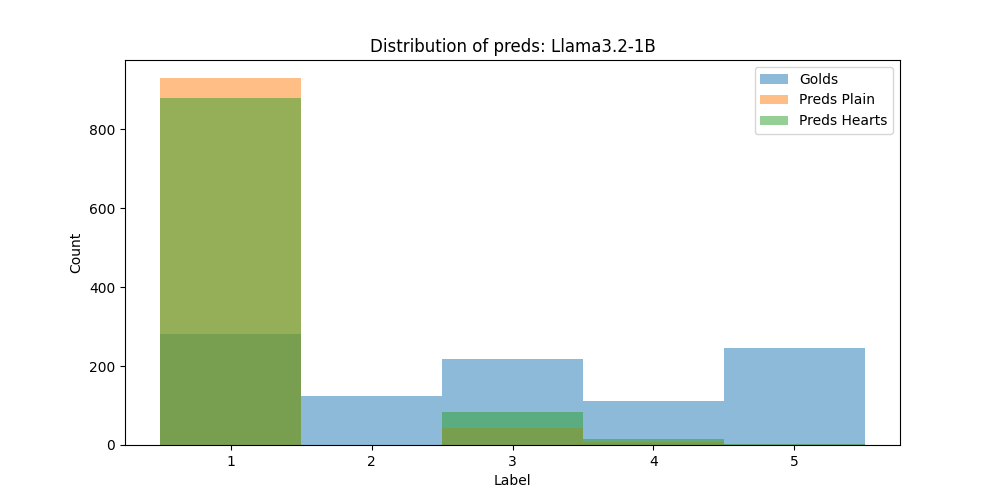
\includegraphics[width=0.7\textwidth]{plots/speaker_experiment/llama3.2-1B_distribution}
    \caption{\textbf{Distribution of predictions on the Speaker Experiment for Llama3.2-1B.}}
    \label{fig:exp2-overall}
\end{figure*}

First, we inspected the overall distributions of the responses from the human participants and the LM and ran a Chi-squared test over the LM outputs (both in hearts and plain modes) against the human data as the reference. As expected, the samples do not come from one distribution, with the p-value approximating $0$ for both tests. The difference between the samples is further attested by the Cohen's Kappa test, with the inter-rater agreement being close to random with the kappa values of 0.028 and 0.006, respectively. Since the data in the hearts mode reached a higher inter-rater agreement, we take it for the further analysis. In the further experimentations excluded from this paper, we found out that the plain mode data had equal or lower statistical effects than the hearts mode data.

The distribution of the \textit{indirect} responses was then investigated following the original procedures from \citet{achimova-2025}. That included:

\begin{itemize}
    \item Investigating the effect of opinions match/mismatch on the proportions of indirect speech with respect to the conversational goals.
    \item Investigating the effect of speaker's opinion on the proportions of indirect speech in the opinion mismatch setting with respect to the conversational goals.
\end{itemize}

By indirect speech, responses that are not faithful to the true opinion of the speaker are understood.

For the former, we aggregated the LM's outputs into samples by match/mismatch and goal properties, calculated the proportions of indirect speech within the samples, and compared the proportions of samples of the same goal when the opinions match/mismatch. The proportions were compared with the two-proportion z-test.

As it can be seen in Figure \ref{fig:exp2-match}, the proportion of indirect speech in the mismatch setting is visually higher than in the match situation, which is in line with the key finding of \citet{achimova-2025}. This effect, is however, insignificant, and we thus conclude that Llama3.2-1B does not exhibit the human tendency to avoid the conflict. We report the respective z-statistic and p-values in Table \ref{table:exp2-match}, where $N$ stands for "total" and $P_i$ for "proportion of indirect speech".

\begin{figure*}[t]
    \centering
    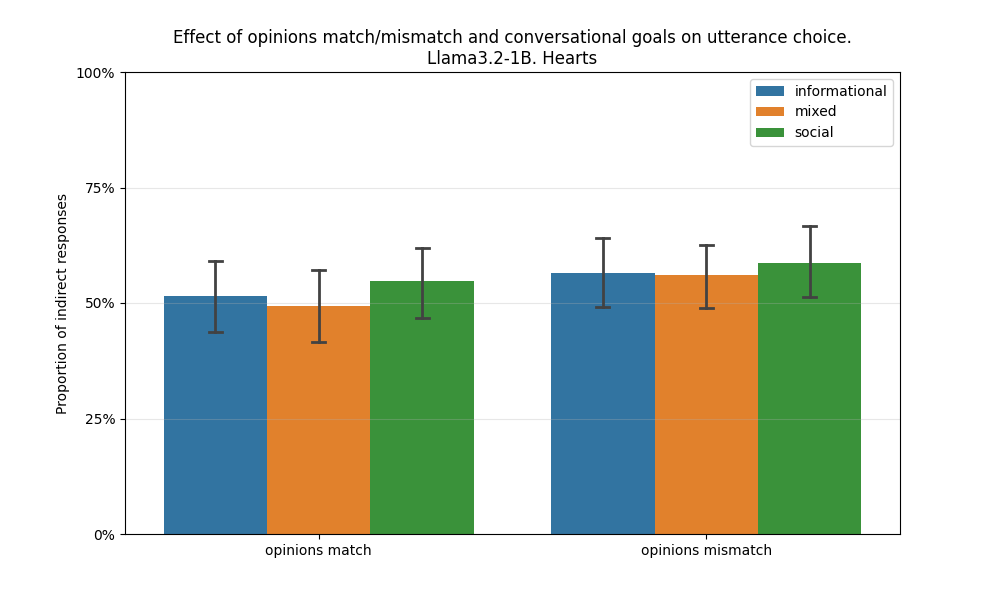
\includegraphics[width=0.7\textwidth]{plots/speaker_experiment/llama3.2-1B_match.png}
    \caption{\textbf{Effect of opinions match/mismatch and conversational goals on utterance choice.}}
    \label{fig:exp2-match}
\end{figure*}

\begin{table*}[t]
    \centering
    \begin{tabular}{lcccccc}
        \toprule
        \textbf{Goal} & \textbf{$N$, Match} & \textbf{$P_i$, Match} & \textbf{$N$, Mismatch} & \textbf{$P_i$, Mismatch} & \textbf{Z} & \textbf{P-value} \\
        \midrule
        Social & 150 & 0.547 & 162 & 0.586 & -0.708 & 0.479 \\
        Mixed & 154 & 0.494 & 184 & 0.560 & -1.216 & 0.224 \\
        Informational & 169 & 0.515 & 161 & 0.565 & -0.919 & 0.358 \\
        \bottomrule
    \end{tabular}
    \caption{Z-statistics and p-values for the effect of opinions match/mismatch on the proportion of indirect responses by conversational goal.}
    \label{table:exp2-match}
\end{table*}


Since the LM mostly produced 1's, it is expected that its answers will mostly be considered as direct if the speaker's opinion is negative, indirect otherwise. This is confirmed by the proportions of the indirect speech when the speaker's and the listener's mismatch, as demonstrated in Figure \ref{fig:exp2-pol}. However, an interesting pattern can be seen in model responses, when the speaker's opinion is strongly negative. The number of indirect responses there visibly grows from informational to social goal, which again corresponds to the findings. Two-proportion z-test between these two polar goal reveals that there is a significant difference between the two proportions, with z-statistic of 2.81 and p-value of 0.005. We thus conclude that Llama3.2-1B exhibits the very beginning of the tendency acquisition, which surfaces in this specific setting.

\begin{figure*}[t]
    \centering
    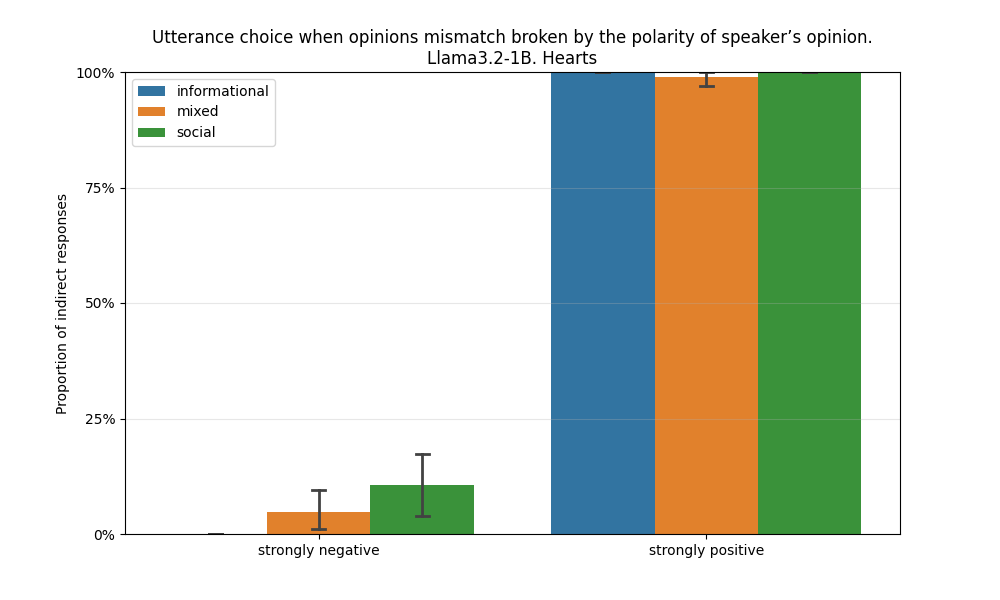
\includegraphics[width=0.7\textwidth]{plots/speaker_experiment/llama3.2-1B_polarity.png}
    \caption{\textbf{Effect of speaker's opinion and conversational goals on utterance choice in the opinions mismatch setting.}}
    \label{fig:exp2-pol}
\end{figure*}



\subsection{Pragmatic Listener Experiment}

Our replication of the pragmatic listener experiment shows a dependency on model size for successful social inference. The small models fail to recognize the nuances of human interaction output. We fail to get a negative monotonic slope, especially in the small language models, though the mid-sized model is more promising in detecting the conflicting context.

% \begin{figure}[h]
%     \centering
%     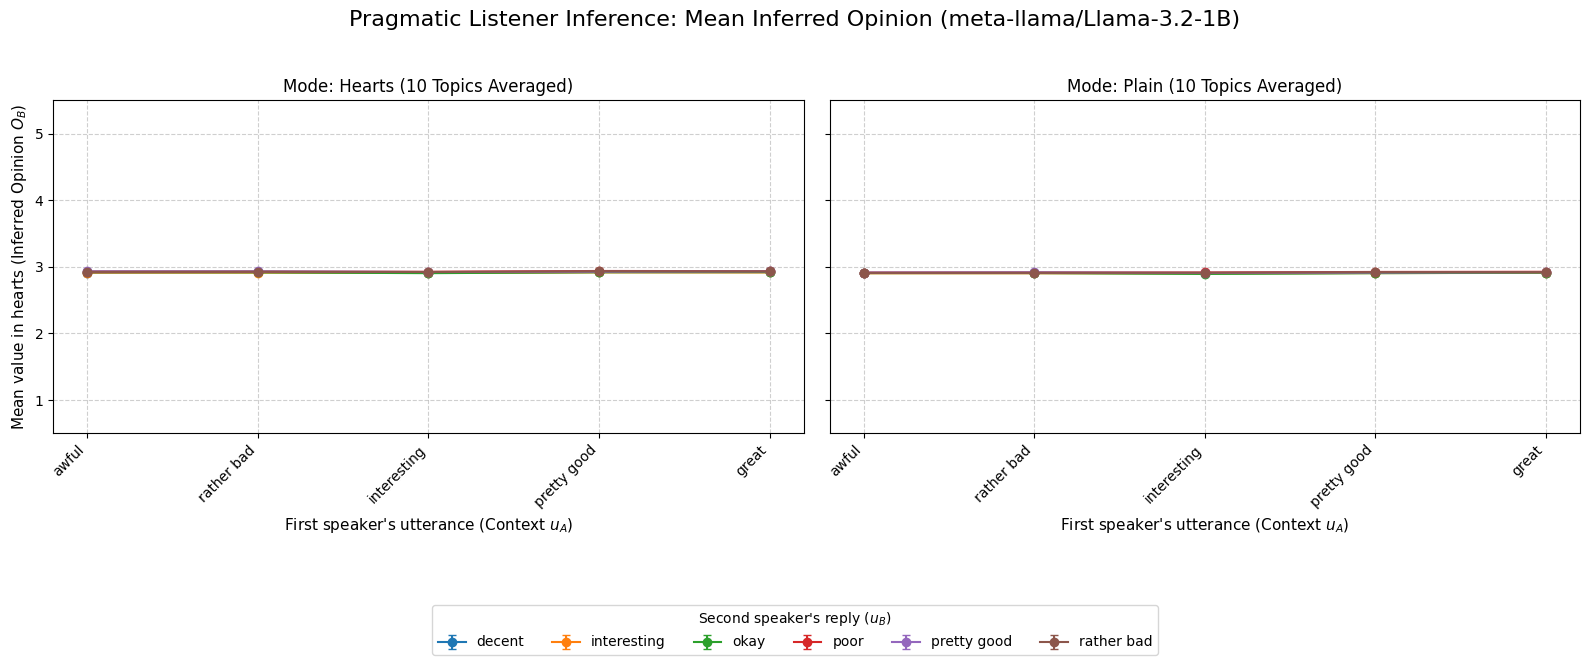
\includegraphics[width=0.7\textwidth]{plots/llama_aggregated.png} \\[1em]
%     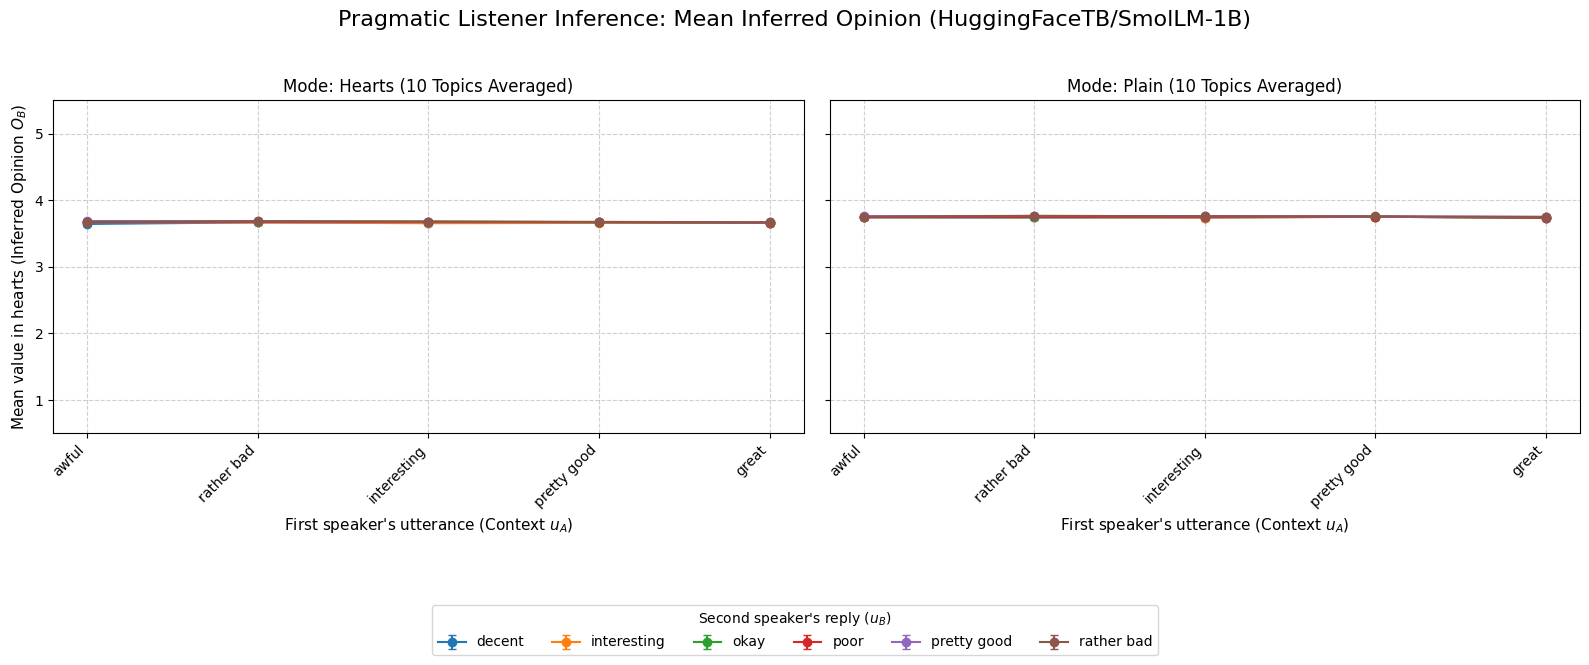
\includegraphics[width=0.7\textwidth]{plots/smol1b_aggregated.png} \\[1em]
%     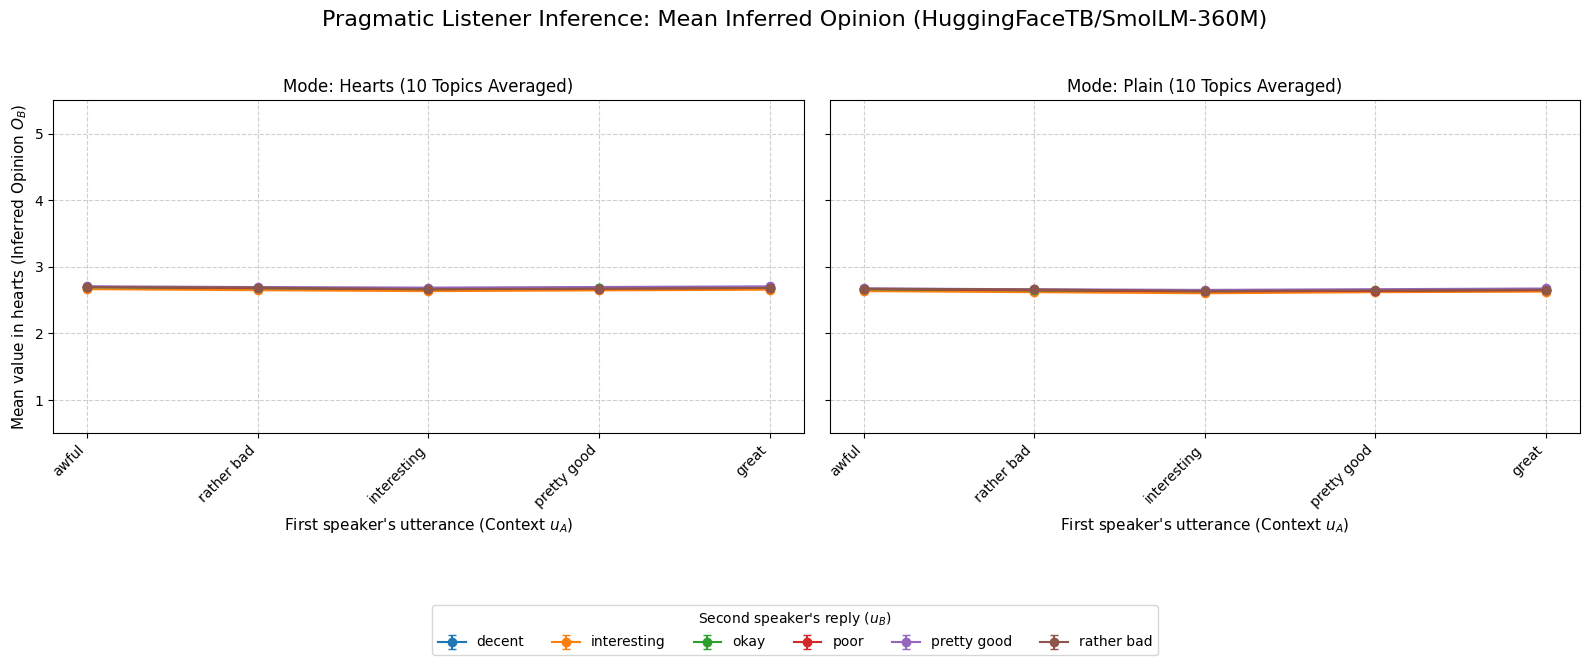
\includegraphics[width=0.7\textwidth]{plots/smol360_aggregated.png}
%     \caption{Lorem Ipsum.}
%     \label{fig:aggregated-plots}
% \end{figure}

\begin{figure*}[t]
    \centering
    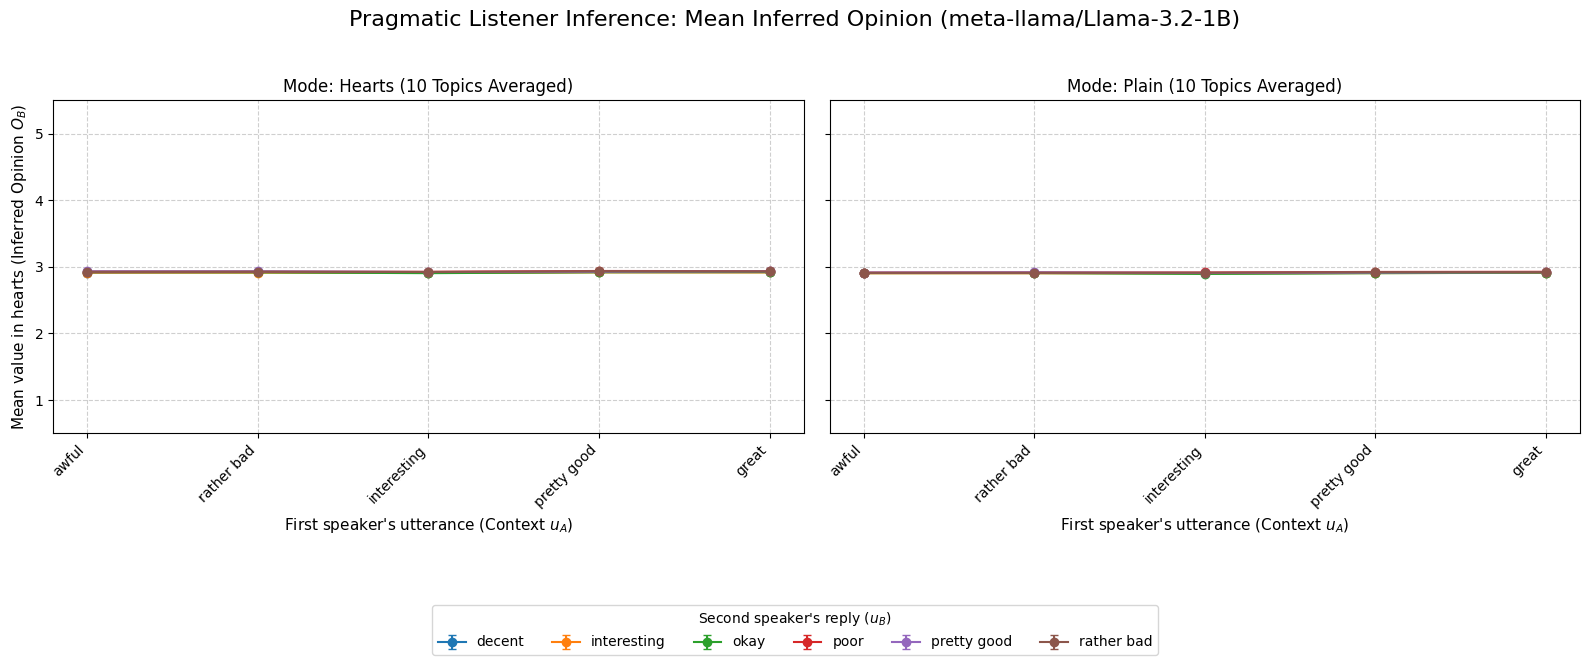
\includegraphics[width=0.7\textwidth]{plots/llama_aggregated.png} \\[1em]
    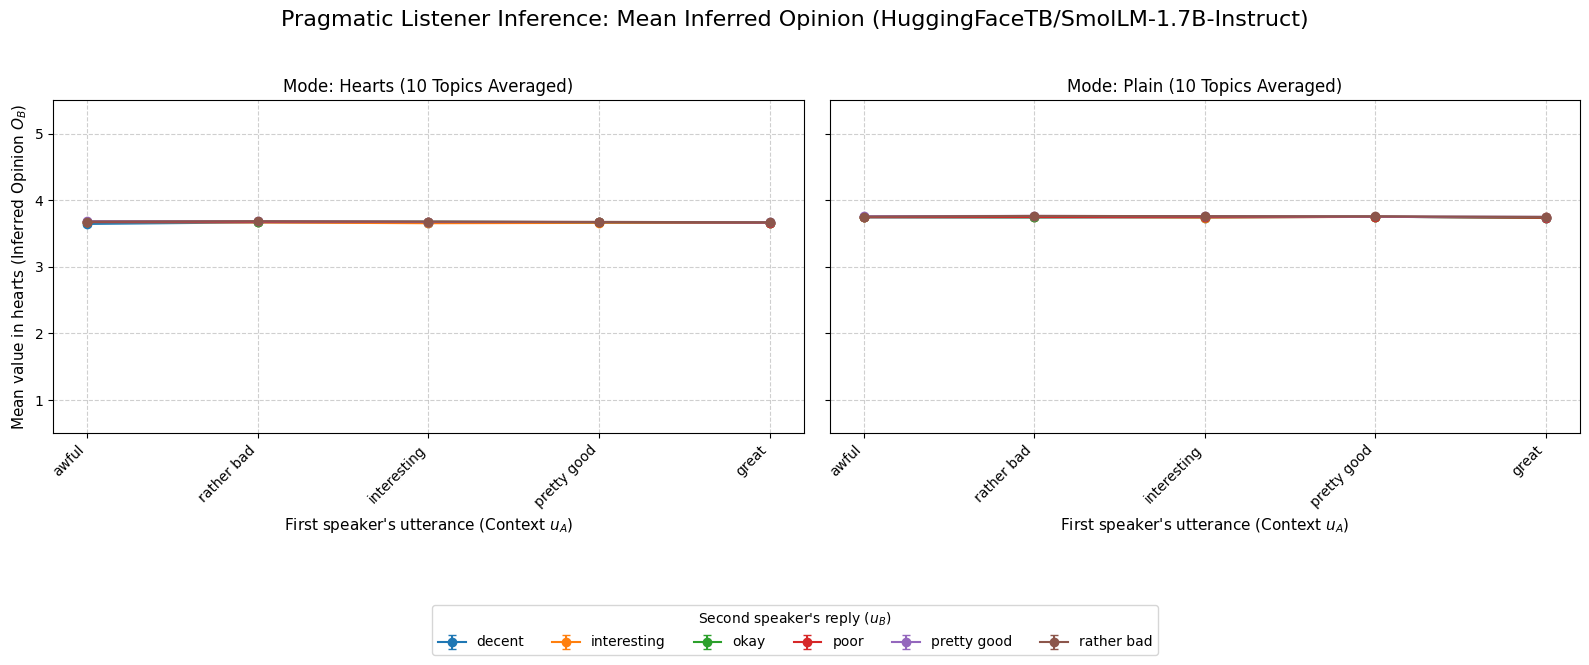
\includegraphics[width=0.7\textwidth]{plots/smol1.7b_aggregated.png} \\[1em]
    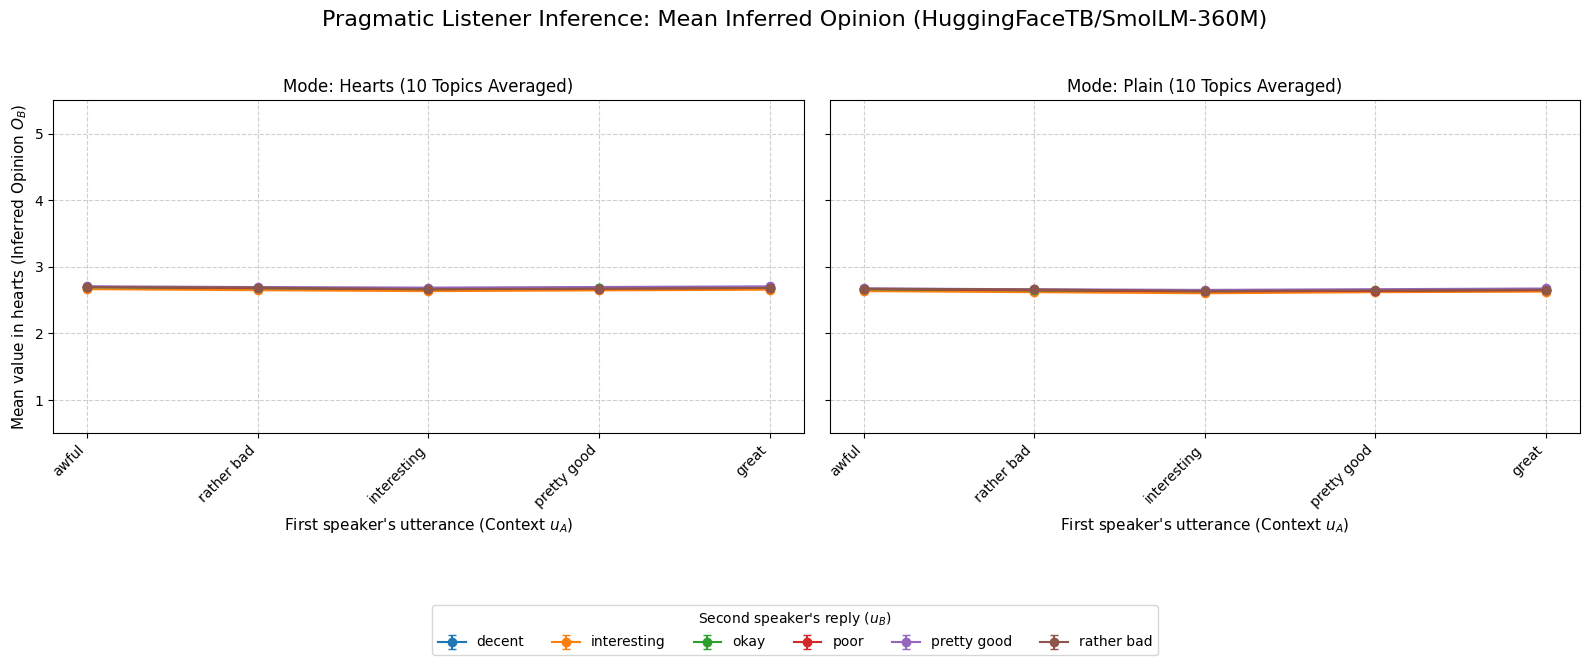
\includegraphics[width=0.7\textwidth]{plots/smol360_aggregated.png}
    \caption{\textbf{Pragmatic Listener Inference Failure in Small Language Models}. The plots display the Mean Inferred Opinion (Y-axis) for three small models, aggregated across all 10 topics and both aesthetic modes (Plain and Hearts). The X-axis represents the Context ($u_{A}$) set by the First Speaker (Awful to Great). The required human behavior is a steep negative monotonic slope. The models prioritize a fixed internal state over linguistic context. This shows a lack of complex social inference capacity in smaller architectures.}
    \label{fig:aggregated-plots}
\end{figure*}


\subsubsection{Analysis of Small-Sized Models (Llama 3.2B and Smol-LLMs)}

The small models tested failed to replicate the fundamental human finding - the \textit{negative monotonic slope} observed in the original experiment---by demonstrating systematic biases that effectively render their output useless for this task. The overview of the performance of small language models can be seen in the figure~\ref{fig:aggregated-plots}

\paragraph{Neutrality Bias}
Llama 3.2-1B consistently returned an inferred answer of 3 (Neutral) \ref{fig:aggregated-plots}. Analysis of the Mean Inferred Opinion confirmed the flat-line behavior observed in the plots. This indicates that the model's core directive to ``avoid conflict'' completely overrides the linguistic evidence ($u_A$ context) and the need to infer the hidden truth. The Llama model defaults to the mathematically safest, non-committal response ($\approx 2.95$), demonstrating a failure of the $L_2$ (Pragmatic Listener) layer.

\paragraph{Polar Bias}
SmolLLM 360M shows a consistent and even stronger tendency toward negativity than Llama, clustering its belief with a flat line at $\approx 2.65$ (figure~\ref{fig:aggregated-plots}). This indicates a pragmatic understanding failure driven by a fixed internal model state. 
SmolLLM 1.7B adopts a strong fixed positive bias, clustering around score 4 (flat line at $\approx 3.7$, Figure~\ref{fig:aggregated-plots}). This is another form of non-contextual failure, where the LLM is unable to perform any required inference.

The smallest models universally failed the core pragmatic task by adopting systematic, non-contextual biases.

\subsubsection{Analysing Mid-Sized Models: Signs of Life and Hope (Qwen 4B)}
\begin{figure*}[h] % h = here, t = top, b = bottom, p = page
    \centering
    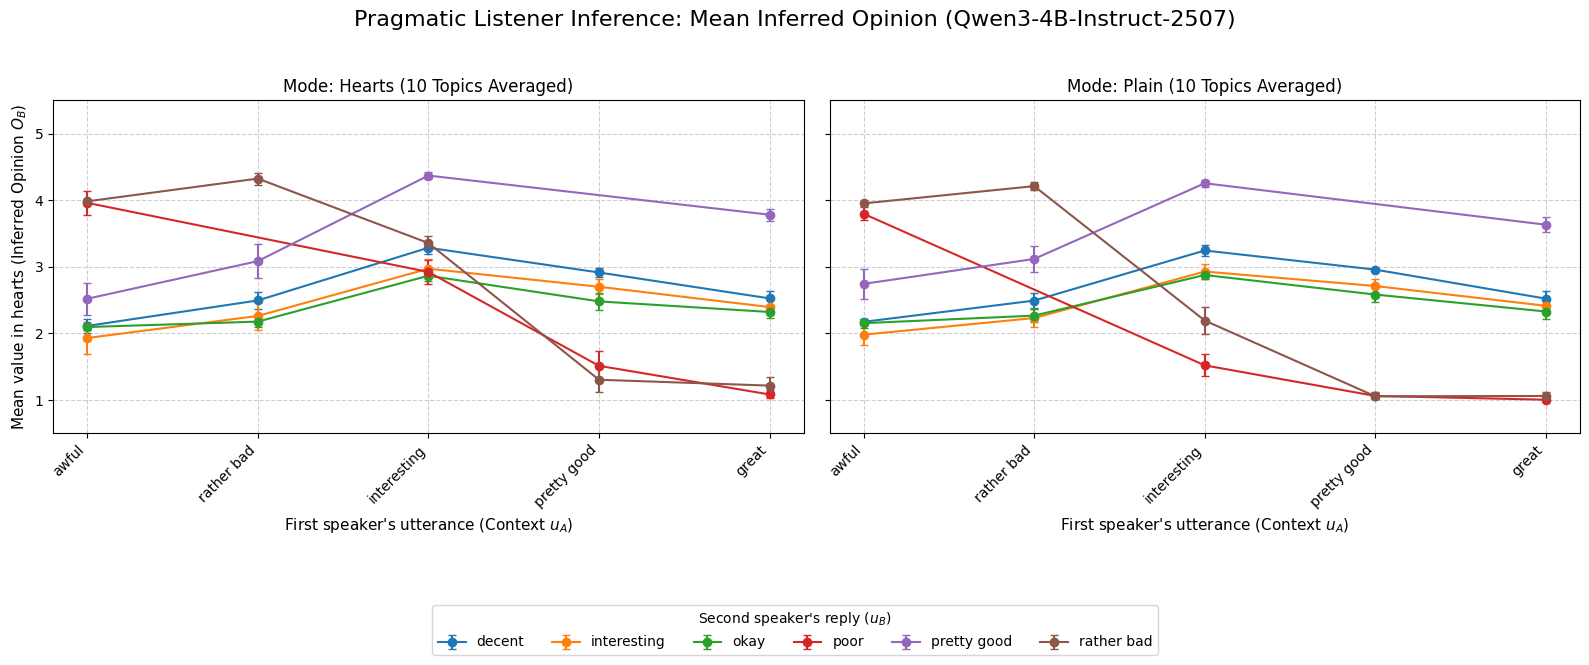
\includegraphics[width=0.7\textwidth]{plots/qwen_aggregated_topics.png}
    \caption{\textbf{Finding:} Qwen 4B breaks the rigid flat-line bias seen in smaller models, proving it possesses the \textbf{capacity to detect and process contextual conflicts}. However, the model fails to execute the pragmatic calculation correctly. Instead of the required negative slope, we see mostly positive slopes, the lines exhibit erratic, steep fluctuations and sudden drops (e.g., the red and brown lines even though they possess negative slopes, suddenly to score 1 rather than a stable downward steps). This behavior confirms a state of \textit{Pragmatic Instability}, where the $L_{2}$ reasoning capacity has emerged but is prone to significant errors, confirming the difficulty of this social inference task at the mid-model scale.}
    \label{fig:llama-plot}
\end{figure*}

The Qwen 4B model demonstrates a qualitative leap: it breaks the rigid flat-line bias and shows an ability to perform highly variable, though often incorrect, contextual calculations.

The model successfully detects and processes the conflicting context ($u_A$) and reply ($u_B$) but lacks the robust hierarchical reasoning to resolve the conflict correctly. The erratic curves confirm it is actively attempting the complex $L_2$ calculation but failing randomly, in an attempt to assess the true belief, leading to a high error rate.

Many per-topic panels show non-zero slopes, proving the model is \textit{trying} to shift its belief based on $u_A$. However, these slopes frequently run in the wrong direction (e.g., they exhibit a positive correlation instead of the required negative one) or are extremely erratic, unlike the lines that human data shows \cite{achimova-2025}, leading to instability.

\begin{figure*}[p] % h = here, t = top, b = bottom, p = page
    \centering
    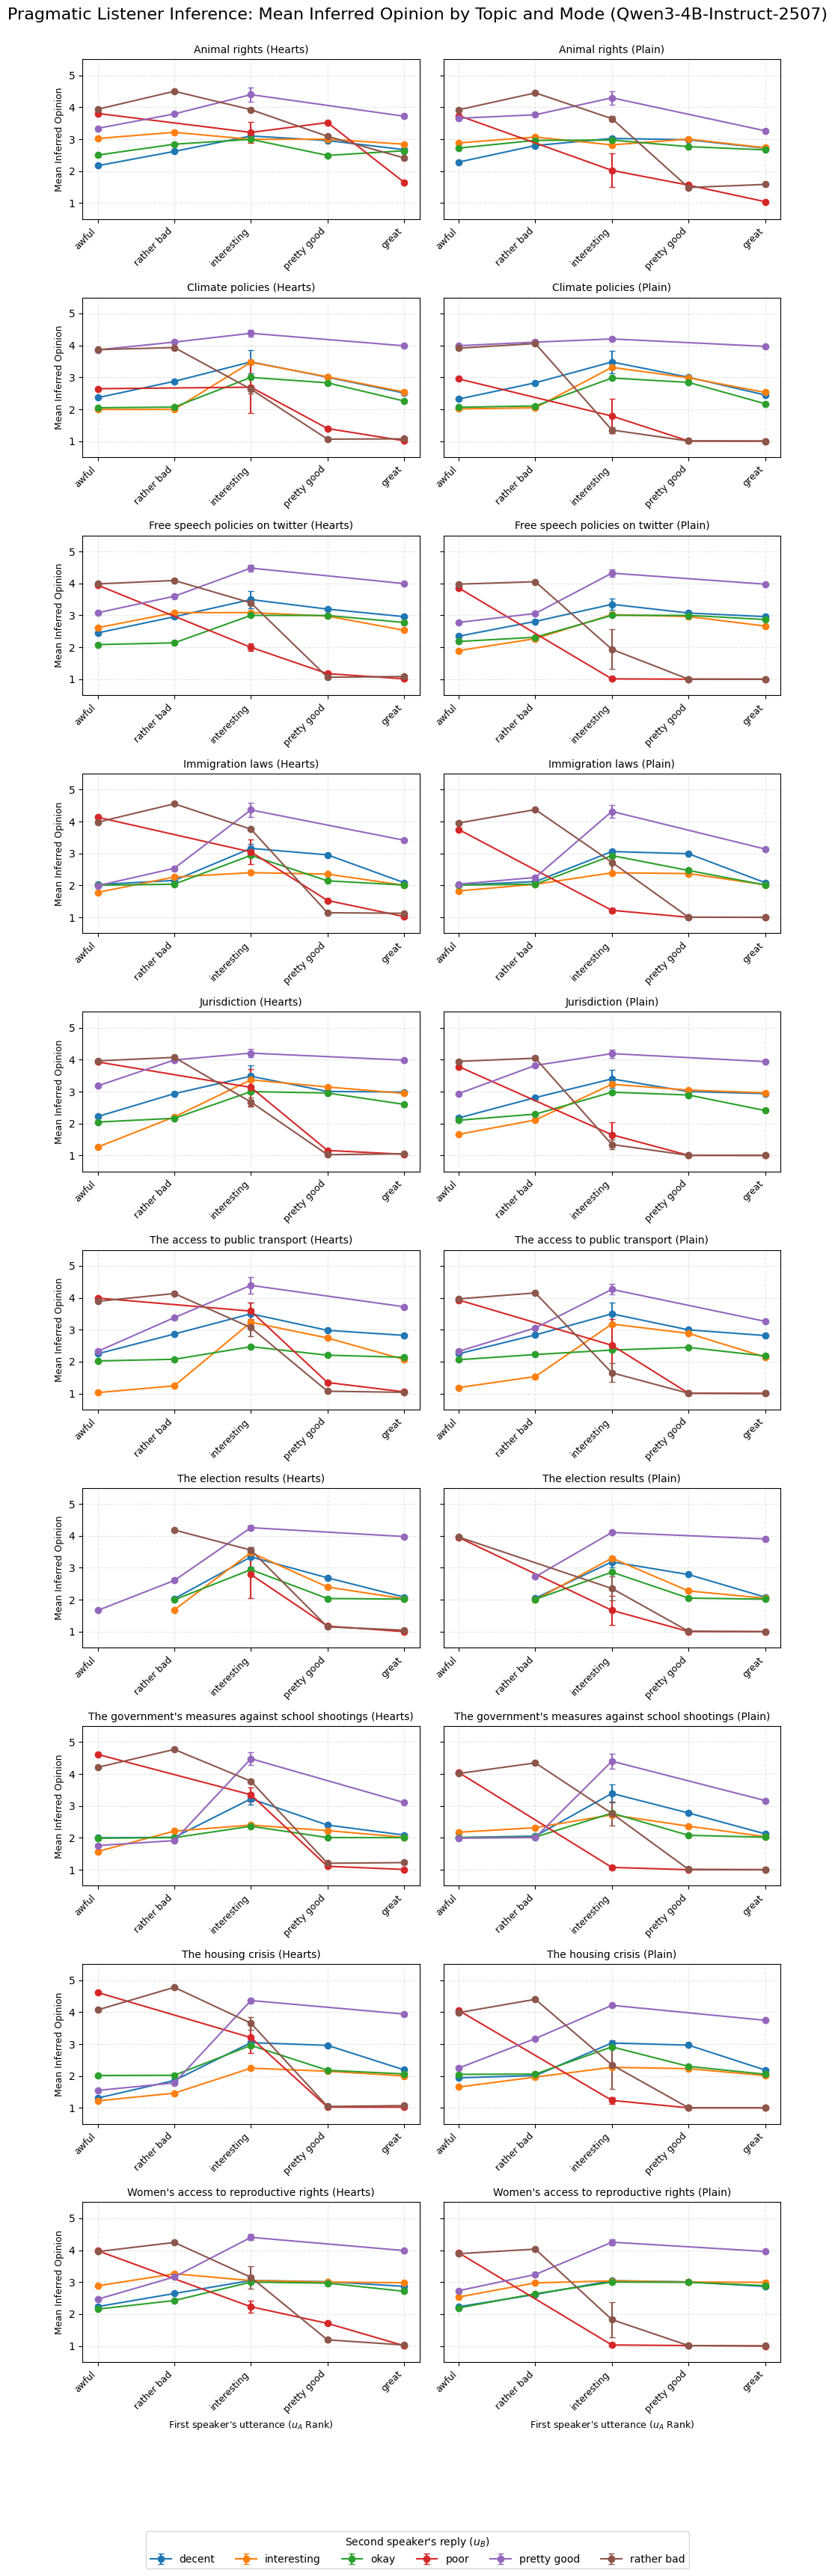
\includegraphics[width=0.5\textwidth]{plots/qwen_per_topic.png}
    \caption{The plots show the Mean Inferred Opinion (Y-axis) for Qwen 4B across 10 topics. Unlike smaller models (Llama, SmolLLM), Qwen breaks the flat-line bias and shows high variability, indicating some capacity to detect conflicting social context. However, most lines are erratic and non-monotonic, revealing a lack of robust hierarchical reasoning for reliable social inference even at this scale.}
    \label{fig:qwen-aggregated-plot}
\end{figure*}

This indicates that at the 4B parameters mark, the reasoning capacity is emerging but still prone to noise and error, confirming that complex social inference is a highly scale/parameter-dependent capability.

\begin{figure*}[t] % h = here, t = top, b = bottom, p = page
    \centering
    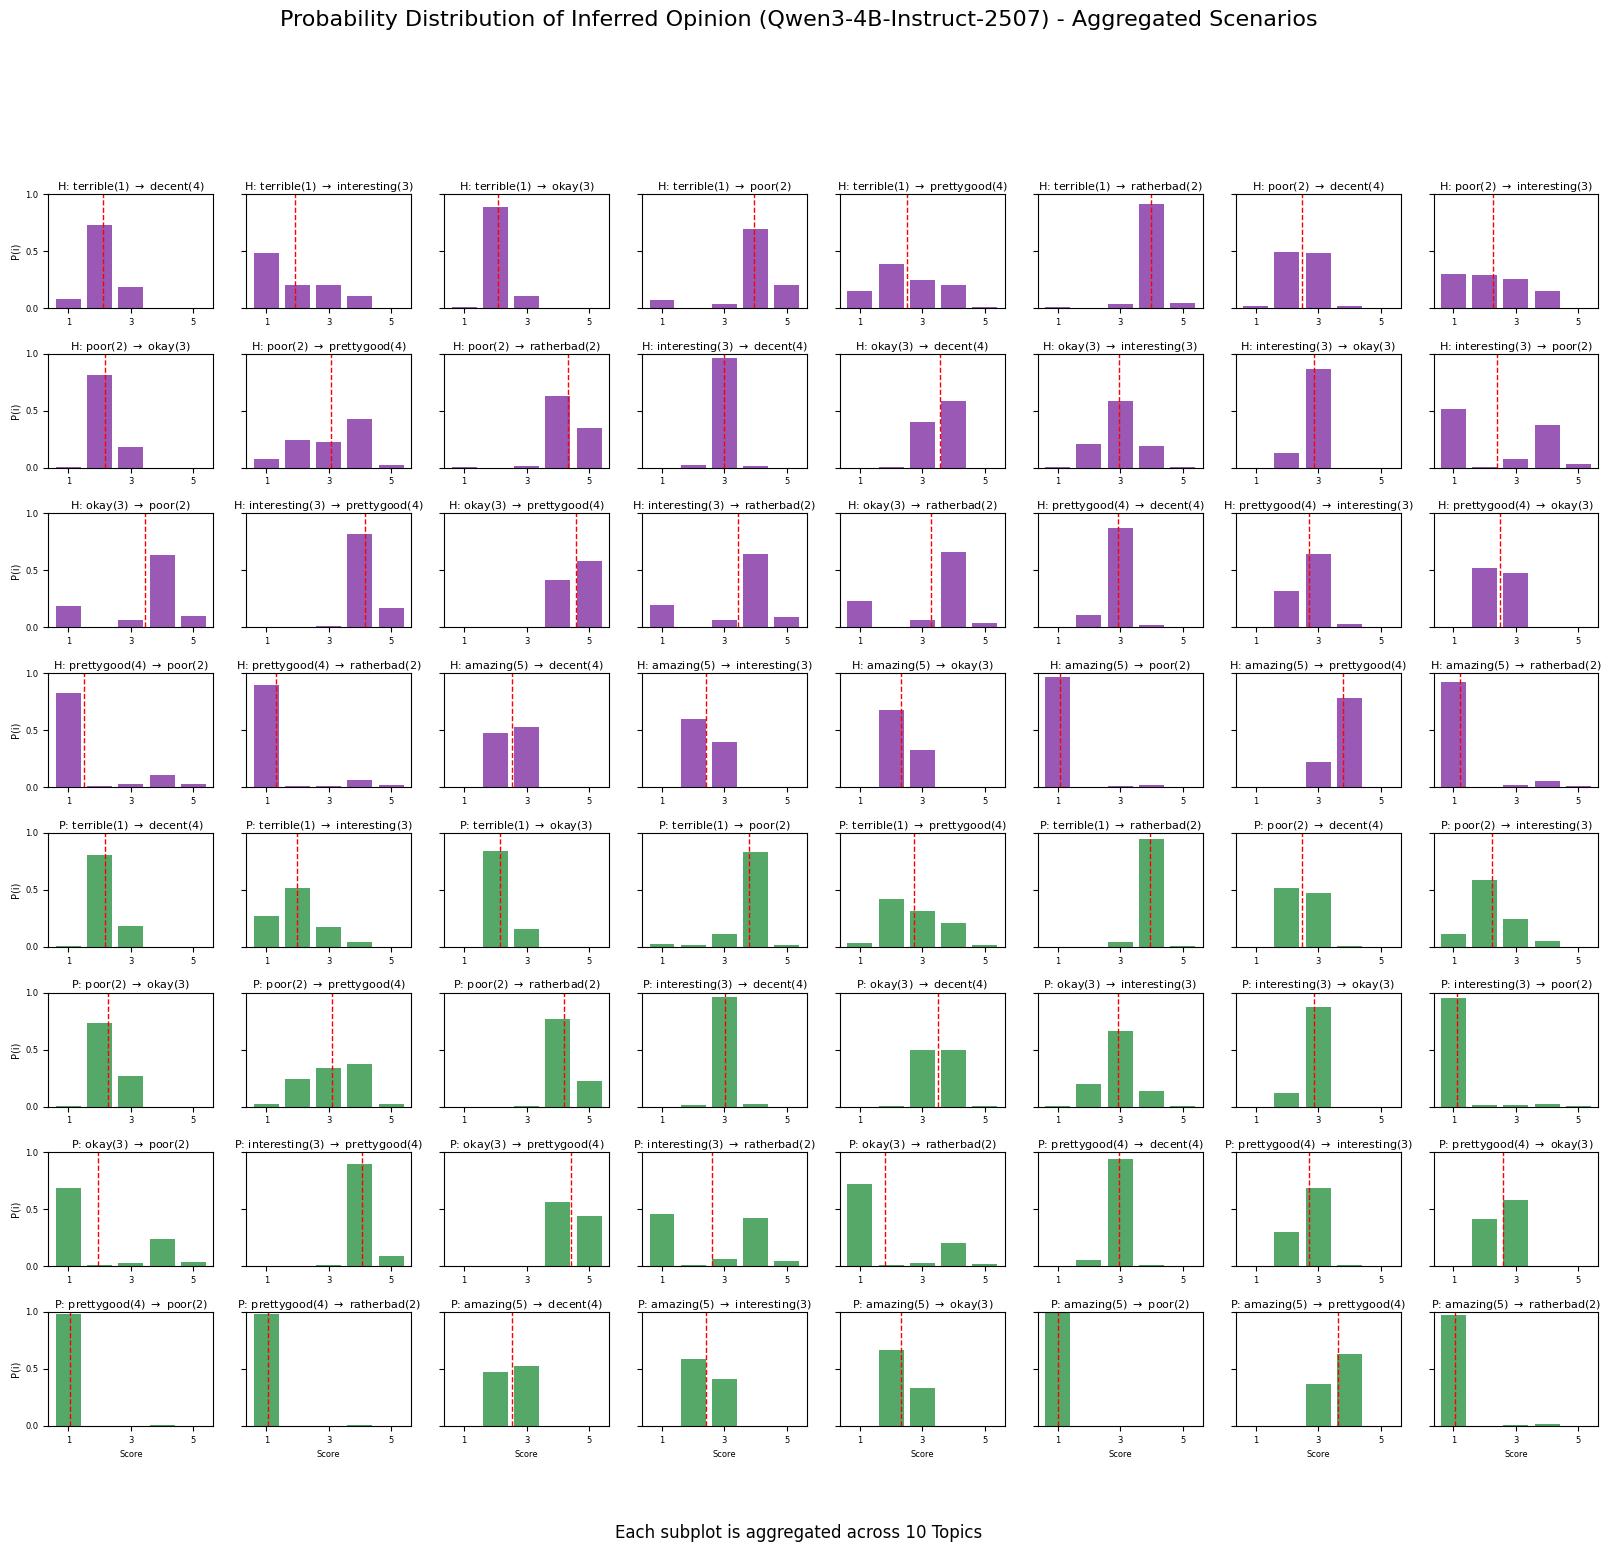
\includegraphics[width=0.7\textwidth]{plots/qwen_log_prob.png}
    \caption{\textbf{Purple: with hearts; Green: Plaintext}
    The grid displays the average probability distribution ($P_i$) for every unique scenario, aggregated across all 10 topics. The red dashed line marks the Mean Inferred Opinion. Labels denote the topic name and the rank (integer score) of $u_a$ and $u_b$. }
    \label{fig:qwen-log-prob}
\end{figure*}


\section{Discussion \& Conclusion}
...

PLAN
1. Summary: small ones such, bigger better. 
2. Hypothesis: small ones are bad because they cannot handle longer contexts and fall for an intermediate option, e.g. the first or the last one
3. SmolLM fucks up always, Llama3.2 shows a small bit of tendency (see in the end of 3.1), Qwen3 is much better ==> Hypothesis: we anticipate that big models will exhibit the tendency
4. Due to the limitations on compute resources, we now limit ourselves to these small models, but it would be interesting to expend the study in a further iteration. 

FINALLY:
1. clean repo
2. pull
3. update README with an instruction to run your exp
4. put src and PDF to the repo
5. push
6. submit



\section*{Acknowledgements}

 We cordially thank our supervisors Dr. Asya Achimova and Polina Tsvilodub for the support and transparent communication thoughout the project. We appreciate the collected experience and hope for future collaborations.


\bibliographystyle{acl_natbib}
\bibliography{custom}


\newpage % Starts a new page for the Appendix

\appendix
\section{Prompt Examples}
\label{sec:appendix:prompts}

Below are examples of the prompts for our LM experiments.

\subsubsection*{Speaker. Plain Text}
\promptblock{
int: The opinions will be written in a plain text, from "strongly negative" to "strongly positive". 

Start!
===========================

Christian wants to discuss the housing crisis with John.
Christian feels strongly positive about the issue.
Christian thinks that John feels strongly positive about it, but he is not sure.

Christian wants to avoid possible conflicts. What would Christian say?

A: The mayor's decision about the housing crisis is awful.
B: The mayor's decision about the housing crisis is rather bad.
C: The mayor's decision about the housing crisis is okay.
D: The mayor's decision about the housing crisis is decent.

===========================

Your answer is 
}

\subsubsection*{Pragmatic Listener. Hearts}
\promptblock{
You are an expert pragmatic listener participating in a linguistic experiment.

In the experiment, small dialogues of two persons on a certain topic will be given to you.

The speakers' goal is always to be polite and avoid conflict, which means their literal words may be INDIRECT and hide their actual, stronger feelings.

Opinion Scale: 1 (Strongly Negative) to 5 (Strongly Positive).

Hint: When thinking about the response, consider that a scale is used:
Strongly Negative (1) $\heartsuit \Box \Box \Box \Box$
Somewhat Negative (2)$\heartsuit \heartsuit \Box \Box \Box$
Neutral (3) $\heartsuit \heartsuit \heartsuit \Box \Box$
Somewhat Positive (4)$\heartsuit \heartsuit \heartsuit \heartsuit \Box$ 
Strongly Positive (5) $\heartsuit \heartsuit \heartsuit \heartsuit \heartsuit$

Your task is to infer the true, underlying opinion of the second person.

You MUST output a single integer from 1 to 5.

Start Inference Task!
===========================
Ethan and Rick meet outside of a club for the first time.
They would like to exchange opinions but don't want to run into a conflict.

Ethan says: The jurisdiction in our district is pretty good.
Rick replies: I find it okay.

How may Rick actually feel about the issue?
Output a single integer between 1 to 5. (1=Strongly Negative, 5=Strongly Positive) 
showcasing the true belief of Rick.
===========================

Your Answer: 
}

% \subsubsection*{B. Plain Text Mode Prompt Example}
% \promptblock{
% You are an expert pragmatic listener participating in a linguistic experiment.

% In the experiment, small dialogues of two persons on a certain topic will be given to you.

% The speakers' goal is always to be polite and avoid conflict, which means their literal words 
% may be INDIRECT and hide their actual, stronger feelings.

% Opinion Scale: 1 (Strongly Negative) to 5 (Strongly Positive).

% Hint: When thinking about the response, consider that a scale is used:
% Strongly Negative (1) 
% Somewhat Negative (2) 
% Neutral (3) 
% Somewhat Positive (4) 
% Strongly Positive (5)

% Your task is to infer the true, underlying opinion of the second person.

% You MUST output a single integer from 1 to 5.

% Start Inference Task!
% ===========================
% Ethan and Rick meet outside of a club for the first time.
% They would like to exchange opinions but don't want to run into a conflict.

% Ethan says: The jurisdiction in our district is terrible.
% Rick replies: I find it rather bad.

% How may Rick actually feel about the issue?
% Output a single integer between 1 to 5. (1=Strongly Negative, 5=Strongly Positive) 
% showcasing the true belief of Rick.
% ===========================

% Your Answer:
% }

\end{document}




\subsubsection{Original Experiment: Goals and Design}

The original experiment in the paper by (asya) titled "Pragmatic Listener" aimed to test the AMIC model’s opinion inference capabilities. The experiment was designed to empirically assess the predictions of the AMIC model’s Pragmatic Listener ($L_{2}$) layer regarding how people infer a speaker's actual, latent opinion after observing a two-turn dialogue. The core goal was to verify whether conversational context and perceived communicative goals dynamically influence the interpretation of an utterance.

Human participants ($n=274$) were presented with a two-turn dialogue between two individuals whose explicit goal was to exchange opinions but avoid conflict (activating the model's social utility). An example of that two turn dialogue presented to the human participants is presented in image xx. The design manipulated the positivity of the First Speaker's Utterance ($u_{1}$) across the scale, and the Second Speaker's Response ($u_{2}$) used neutral to slightly positive/negative indirect terms. The experiment checked a key monotonicity prediction: that the inferred opinion of $S_{2}$ for a fixed response ($u_{2}$) would be \textbf{negatively correlated} with the positivity of the preceding statement ($u_{1}$). This confirmed that human interpretation dynamically adjusts to the social context of conflict avoidance. 

The hardware used for this experiment was Apple Silicon CPU (M4 10 core) on a Macbook Air 2025. The inference pipeline was built on the same inference engine used in the Pragmatic Speaker experiment, ie, vLLM API Server. The concurrency limit was set to match the observed stable CPU core saturation, and the timeout was increased to 3600s to prevent frequent failures caused by long CPU batch processing times. Apart from that, the temperature was set to 0.001 (Maxed to 0.01 by vLLm server) to ensure the model's output is highly deterministic (non-random) for reliable measurement of the highest-probability pragmatic decision.